\iffalse
\documentclass[12pt]{article}
\usepackage{graphicx}
\usepackage{amsmath}
\usepackage{mathtools}
\usepackage{gensymb}

\newcommand{\mydet}[1]{\ensuremath{\begin{vmatrix}#1\end{vmatrix}}}
\providecommand{\brak}[1]{\ensuremath{\left(#1\right)}}
\providecommand{\norm}[1]{\left\lVert#1\right\rVert}
\newcommand{\solution}{\noindent \textbf{Solution: }}
\newcommand{\myvec}[1]{\ensuremath{\begin{pmatrix}#1\end{pmatrix}}}
\let\vec\mathbf

\begin{document}
\begin{center}
\textbf\large{CHAPTER-7 \\ COORDINATE GEOMETRY}
\end{center}
\section*{Excercise 7.1}

Q1. Find the distance between the following pairs of points :
\begin{enumerate}
	\item $\brak{2,3}, \brak{4,1}$ 
	\item $\brak{-5,7}, \brak{-1,3}$
	\item $\brak{a,b}, \brak{-a,-b}$
\end{enumerate}
\fi
\solution
\begin{enumerate}
\item The coordinates are given as
	\begin{align}
	\vec{A} = \myvec{
		2\\
		3\\
		},
		\vec{B} &= \myvec{
		4\\
		1\\
		}
		\\
\implies		\vec{A} - \vec{B} = \myvec{2\\3} - \myvec{4\\1} &= \myvec{-2\\2}		
\\
		\implies		(\vec{A}-\vec{B})^\top (\vec{A}-\vec{B}) &= 8
	\end{align}
	Thus, the desired distance is 
	\begin{align}
		d=\norm{\vec{A}-\vec{B}} =\sqrt{8}
	\end{align}
	See Fig. \ref{fig:10/7/1/1Fig}.
\item The coordinates are given as
	\begin{align}
	\vec{C} = \myvec{
		-5\\
		7\\
		},
		\vec{D} &= \myvec{
		-1\\
		3\\
		}
\implies		\vec{C} - \vec{D} = \myvec{-5\\7} - \myvec{-1\\3} &= \myvec{-4\\4}		
		\\
		\implies		(\vec{C}-\vec{D})^\top (\vec{C}-\vec{D}) &= 32
	\end{align}
Thus,	
	\begin{align}
		d=\norm{\vec{C}-\vec{D}}
 =4\sqrt{2}
\end{align}	
	See Fig. \ref{fig:10/7/1/1Fig}.
%	
\item The coordinates are given as
	\begin{align}
	\vec{E} = \myvec{
		a\\
		b\\
		},
		\vec{F} &= \myvec{
		-a\\
		-b\\
		}
		\implies		\vec{E} - \vec{F} = \myvec{a\\b} - \myvec{-a\\-b} &= \myvec{2a\\2b}		
		\\
		\implies
		(\vec{E}-\vec{F})^\top (\vec{E}-\vec{F}) = 4a^2+4b^2 
	\end{align}
Thus,	
	\begin{align}
		d=\norm{\vec{E}-\vec{F}} =
2\sqrt{a^2+b^2}
\end{align}	
See  
Fig. \ref{fig:10/7/1/1Fig} for 
$ a=1,b=2$ 
\begin{figure}[!h]
	\begin{center} 
	    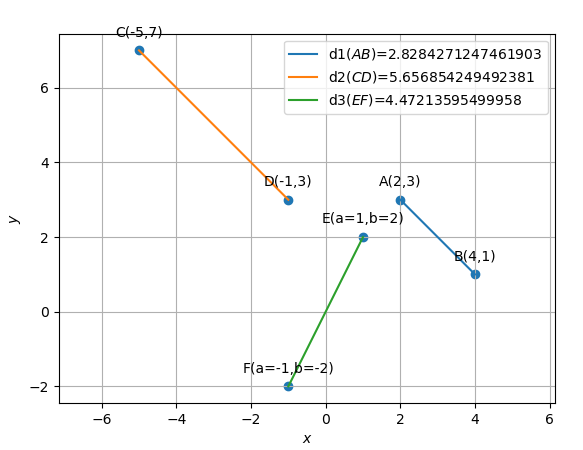
\includegraphics[width=\columnwidth]{chapters/10/7/1/1/figs/graph.png}
	\end{center}
\caption{}
\label{fig:10/7/1/1Fig}
\end{figure}
\end{enumerate}
